\documentclass{article}
\usepackage[utf8]{inputenc}

\usepackage{tikz} 

\usetikzlibrary{positioning} % Required for positioning of nodes

\begin{document}
\noindent \begin{tikzpicture}[node distance = 0pt,
IdxStyle/.style={draw=none, minimum width=2em, minimum height=2em, 
                outer sep=0pt},]
\node [IdxStyle] (l21) {1};
\node [IdxStyle, right=of l21] (r21) {2};
\node [IdxStyle, right=of r21] (l22) {3};
\node [IdxStyle, right=of l22] (r22) {4};
\end{tikzpicture}
\newline
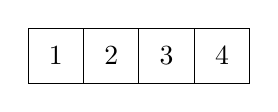
\begin{tikzpicture}[node distance = 0pt,
ItemStyle/.style={draw, minimum width=2em, minimum height=2em, 
                outer sep=0pt},]
\node [ItemStyle] (l21) {1};
\node [ItemStyle, right=of l21] (r21) {2};
\node [ItemStyle, right=of r21] (l22) {3};
\node [ItemStyle, right=of l22] (r22) {4};
\end{tikzpicture}
\newline
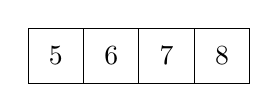
\begin{tikzpicture}[node distance = 0pt,
ItemStyle/.style={draw, minimum width=2em, minimum height=2em, 
                outer sep=0pt},]
\node [ItemStyle] (l21) {5};
\node [ItemStyle, right=of l21] (r21) {6};
\node [ItemStyle, right=of r21] (l22) {7};
\node [ItemStyle, right=of l22] (r22) {8};
\end{tikzpicture}
\end{document}
